\documentclass[pdf,utf8,xcolor=x11names]{beamer}
\usepackage{url}
\usepackage{pgf}
\usepackage{tikz}
\usepackage{listings}
\usepackage{alltt}
\usepackage{xspace}
\usepackage{multirow}
\usepackage{pifont}
\usepackage{array}

\usetheme{frama-c}

\usetikzlibrary{shapes.callouts}
\usetikzlibrary{shapes.geometric}
\usetikzlibrary{fit}

\newcommand{\framacversion}%
           {\input{../../VERSION}\unskip{} (\input{../../VERSION_CODENAME}\unskip)}
\newcommand{\nextframacversion}{Frama-C+dev}

\newcommand{\tool}[1]{\textsf{#1}\xspace}

\newcommand{\C}{\tool{C}}
\newcommand{\caml}{\tool{OCaml}}
\newcommand{\acsl}{\tool{ACSL}\index{ACSL@\tool{ACSL}}}
\newcommand{\gcc}{\tool{GCC}}
\newcommand{\Value}{\tool{Eva}}
\newcommand{\Eva}{\tool{Eva}}
\newcommand{\From}{\tool{From}}
\newcommand{\WP}{\tool{WP}}
\newcommand{\Report}{\tool{Report}}
\newcommand{\Slicing}{\tool{Slicing}}
\newcommand{\GUI}{\tool{GUI}}
\newcommand{\opam}{\tool{opam}}

\newenvironment{commands}%
{\par\hspace{2cm}\begin{tabular}{l}}%
{\end{tabular}}

\newcommand{\via}{\emph{via}\xspace}
\newcommand{\etc}{\emph{etc}\xspace}
\newcommand{\ie}{\emph{i.e.}\xspace}
\newcommand{\eg}{\emph{e.g.}\xspace}

% Index

\newcommand{\optionidx}[2]{\index{#2@\texttt{#1#2}}}
\newcommand{\codeidx}[1]{\index{#1@\texttt{#1}}}
\newcommand{\scodeidx}[2]{\index{#1@\texttt{#1}!#2@\texttt{#2}}}
\newcommand{\sscodeidx}[3]{%
  \index{#1@\texttt{#1}!#2@\texttt{#2}!#3@\texttt{#3}}}
\newcommand{\bfit}[1]{\textbf{\textit{\hyperpage{#1}}}}
\newcommand{\optionidxdef}[2]{\index{#2@\texttt{#1#2}|bfit}}
\newcommand{\codeidxdef}[1]{\index{#1@\texttt{#1}|bfit}}
\newcommand{\scodeidxdef}[2]{\index{#1@\texttt{#1}!#2@\texttt{#2}|bfit}}
\newcommand{\sscodeidxdef}[3]{%
  \index{#1@\texttt{#1}!#2@\texttt{#2}!#3@\texttt{#3}|bfit}}

\newcommand{\pragmadef}[1]{\texttt{#1}\index{Pragma!#1@\texttt{#1}}}
\newcommand{\optiondef}[2]{\texttt{#1#2}\optionidxdef{#1}{#2}}
\newcommand{\deprecatedoptiondef}[2]{\texttt{#1#2}\index{#2@\texttt{#1#2} \textit{Deprecated option}|bfit}}
\newcommand{\textttdef}[1]{\texttt{#1}\codeidxdef{#1}}

\newcommand{\optionuse}[2]{\texttt{#1#2}\optionidx{#1}{#2}}
\newcommand{\textttuse}[1]{\texttt{#1}\codeidx{#1}}

% Special environment
\definecolor{gris}{gray}{0.85}

\makeatletter
\newenvironment{important}%
{\hspace{5pt plus \linewidth minus \marginparsep}%
 \begin{lrbox}{\@tempboxa}%
   \begin{minipage}{\linewidth - 2\fboxsep}}
{\end{minipage}\end{lrbox}\colorbox{gris}{\usebox{\@tempboxa}}}
\makeatother

\newtheorem{convention}{Recommendation}[chapter]


\makeatletter
\AtBeginPart{
\addtocontents{toc}{%
\protect\beamer@partintoc{\the\c@part}{\beamer@partnameshort}{\the\c@page}}%
\begin{frame}
\tableofcontents[currentpart]
\end{frame}
}
\providecommand\beamer@partintoc[3]{%
  \ifnum\c@tocdepth=-1\relax
    % requesting onlyparts.
    \usebeamercolor[fg]{section in toc}{\makebox[6em]{Part #1:} #2}
    \par
    \vfill
  \fi
}
\define@key{beamertoc}{onlyparts}[]{%
  \c@tocdepth=-1\relax
}
\makeatother%

\author{Virgile Prevosto and Julien Signoles\\[2mm]
\texttt{firstname.lastname@cea.fr}}
\institute{
\includegraphics[width=0.15\textwidth]{cealist.pdf}}
\title{Frama-C Plug-in Developer Training}
\date{2012-05-xy}

\begin{document}
\titlepage
\begin{frame}{Overview}
\tableofcontents[onlyparts]
\end{frame}

%%%%%%%%%%%%%%%%%%%%%%%%%%%%%%%%%%%%%%%%%%%%%%%%%%%%%%%%%%%%%%%%%%%%%%%%%%%%%%%
%%%%%%%%%%%%%%%%%%%%%%%%%%%%%%%%%%%%%%%%%%%%%%%%%%%%%%%%%%%%%%%%%%%%%%%%%%%%%%%

\part{First steps}

\section{Gentle \protect\ocaml reminder}

\subsection{Basic features}
%JS:15mn
\begin{frame}[fragile]{\ocaml, a functional language}
  
  \begin{itemize}
  \item \ocaml is a \orangepale{functional language}
  \item functions are first-class values
  \end{itemize}
  \pause
  \begin{alltt}
    \# let l = [ 1; -4; 5; 3 ];;\pause
    \gris{val l : int list = [1; -4; 5; 3]}\pause
    \# List.map (fun x -> x * 2) l;;\pause
    \gris{- : int list = [2; -8; 10; 6]}\pause
    \# List.sort Pervasives.compare l;;\pause
    \gris{- : int list = [-4; 1; 3; 5]}\pause
    \# List.fold\_left ( + ) 0 l;;\pause
    \gris{- : int = 5}
  \end{alltt}
  
\end{frame}

\begin{frame}[fragile]{\ocaml, an imperative language}
  \framesubtitle{Reference and mutable records}

  \begin{itemize}
  \item \ocaml is also an \orangepale{imperative language}
  \item \orangepale{references}
%{\small
    \begin{ocamlcode}
let x = ref 0
let () = x := 3
(* let () = x := "three" *) (* incorrect! *)
let n = !x       (* n is 3 *)
let y = x        (* aliasing *)
let () = x := 2
let m = !y       (* m is 2 *)
    \end{ocamlcode}%}
  \item \orangepale{mutable records}
    \begin{ocamlcode}
type t = { mutable int a; bool b }
let x = { a = 0; b = true; }
let () = x.a <- 1
    \end{ocamlcode}
  \end{itemize}

\end{frame}

\begin{frame}[fragile]{\ocaml, an imperative language}
  \framesubtitle{Printers}

  \begin{itemize}
  \item printers \emph{\`a la} printf (even more powerful)
\begin{ocamlcode}
let three = "three"
let () = Format.printf "%s is %d" three 3

type t = A | B of int
let print fmt = function
  | A -> Format.fprintf fmt "A"
  | B n -> Format.fprintf fmt "B %d" n
let () = 
  List.iter
    (fun x -> Format.printf "%a " print x) 
    [ A; B 3; B (-4) ]
\end{ocamlcode}
  \end{itemize}

\end{frame}

\begin{frame}[fragile]{\ocaml, an imperative language}
  \framesubtitle{Standard imperative datastructures}

  \begin{itemize}
  \item Hashtables
\begin{ocamlcode}
let h = Hashtbl.create 7
let () = 
  List.iter
    (fun (n, s) -> Hashtbl.add h n s)
    [ 1, "one"; 2, "two"; 3, "three" ]
let two = Hashtbl.find h 2
let () = 
  Hashtbl.iter
    (fun (n, s) -> 
      Format.printf "%d --> %s" n s)
    h
\end{ocamlcode}
  \item Array, Stack, Queue
  \end{itemize}
\end{frame}

\begin{frame}[fragile]{\ocaml, an imperative language}
  \framesubtitle{Exception}

    \begin{ocamlcode}
let h = (* hashtbl of the previous slide *)
let four = 
  try Hashtbl.find h 4 
  with Not_found -> "four"

exception Found of string
let mem_value p =
  try
    Hashtbl.iter
      (fun _ s -> if p s then raise (Found s))
      h;
    None
  with Found s ->
    Some s
  \end{ocamlcode}

\end{frame}

\begin{frame}{\ocaml, an imperative language}
\framesubtitle{Summary}

\begin{itemize}
\item sharing and backwards links 
  \begin{itemize}
  \item aliasing
  \item \framac's AST
  \end{itemize}
\item complexity 
  \begin{itemize}
  \item random access in an array \emph{vs} in a list
  \item search in an hashtbl \emph{vs} in a map or a list
  \end{itemize}
\item ease of implementation 
  \begin{itemize}
  \item raising an exception \emph{vs} returning an option type
  \item no need to push an environment across call stack
  \end{itemize}
\end{itemize}

\end{frame}


\subsection{Module system}
\begin{frame}{Module}
  \framesubtitle{Overview}

  \begin{itemize}
  \item small typed functional language by itself
  \item based on the core language
  \item namespace
  \item encapsulation
  \item generic programming
  \end{itemize}

\end{frame}

\begin{frame}[fragile]{Module}
  \framesubtitle{Structure}

  \begin{ocamlcode}
(* implementation of rationals *)
struct
  type t = int * int
  let pgcd n m = ...
  let make n d = 
    let p = pgcd n d in
    n / p, d / p
  let integer n = n, 1
  let add (n1, d1) (n2, d2) = 
    make (n1 * d2 + n2 * d1) (d1 * d2)
  ...
end
  \end{ocamlcode}

\end{frame}

\begin{frame}[fragile]{Module}
  \framesubtitle{Names, submodule and access}

\begin{ocamlcode}
(* modules can be named *)
module Rational = 
  ... (* code of the previous slide *)

(* submodules are possible *)
module M1 = struct 
  module M2 = struct 
    module M3 = struct let x = ... end 
  end 
end

(* access through the dot notation *)
let r_one: Rational.t = Rational.integer 1
let x = M1.M2.M3.x
\end{ocamlcode}
\end{frame}

\begin{frame}[fragile]{Module}
  \framesubtitle{Typing}

  \begin{itemize}
  \item \ocaml infers a module type for each module
  \item types of structure are signatures
  \end{itemize}

  \begin{ocamlcode}
(* inferred type for module Rational *)
sig
  type t = int * int
  val pgcd: int -> int -> int
  val make: int -> int -> int * int
  val integer: int -> int * int
  val add: int * int -> int * int -> int * int
  ...
end
  \end{ocamlcode}
\end{frame}

\begin{frame}[fragile]{Module}
  \framesubtitle{Explicit Signature}

  \begin{ocamlcode}
module type Rational = sig
  type t
  val make: int -> int -> t
  val integer: int -> t
  val add: t -> t -> t
  ...
end
module Rational: Rational
  \end{ocamlcode}

  \begin{itemize}
  \item abstract types
  \item hide implementation details through subtyping
  \item encapsulation: easy to change the implementation without
    changing its interface
  \item unnamed signature
  \end{itemize}

\end{frame}

%% \begin{frame}[fragile]{Module}
%%   \framesubtitle{Compilation Unit}

%%   \begin{itemize}
%%   \item .ml files are particular structures
%%   \item .mli files are particular signatures
%%   \end{itemize}

%%   \begin{ocamlcode}
%% module L = List
%% module C = Cil
%% module type T = Cil_types
%%   \end{ocamlcode}
%% \end{frame}

\begin{frame}[fragile]{Module}
  \framesubtitle{Opening and inclusion}

  \begin{ocamlcode}
open Rational
let r_one = zero
open Cil_types

module My_list = struct
  include List
  let singleton x = [ x ]
  let tl _ = failwith "should never be used"
end
  \end{ocamlcode}

  \begin{itemize}
  \item `\lstinline+open+' provides a direct access to a structure's namespace
    (or signature)
  \item usually bad to have to many `\lstinline+open+' at the same time
  \item `\lstinline+include+' allows to extends/redefine a structure or a
    signature
  \end{itemize}

\end{frame}

\begin{frame}[fragile]{Module}
  \framesubtitle{Functor definition}
  
\begin{ocamlcode}
module type Ring = sig
  type t
  val zero: t         val one: t
  val add: t -> t -> t  val opp: t -> t
  val mult: t -> t -> t
end
module Polynomial(R: Ring) = struct
  type ring = R.t    type t = R.t array
  let zero = [| R.zero |]
  let monomial c n =
    let p = Array.create (n + 1) R.zero in
    p.(n) <- c; p
   ...
end
\end{ocamlcode}
\end{frame}

\begin{frame}[fragile]{Module}
  \framesubtitle{Functor use}

\begin{ocamlcode}
module IntegerPolynomial =
  Polynomial
    (struct
      type t = int
      let zero = 0
      let one = 1
      let add = ( + )
      let mult = ( * )
      let opp n = - n
    end)

module RationalPolynomial = 
  Polynomial(Rational)
\end{ocamlcode}
\end{frame}

\begin{frame}[fragile]{Module}
  \framesubtitle{Functor typing}

\begin{ocamlcode}
module Polynomial(R: Ring) = sig
  type ring = R.t    type t
  val zero: t      
  val monomial: R.t -> int -> t
  ...
end
  
module type Polynomial: sig
  type ring     type t
  val zero: t   val monomial: R.t -> int -> t
end
module Polynomial(R: Ring):
  Polynomial with type ring = R.t
\end{ocamlcode}

\end{frame}

%JS:30mn

\subsection{Object-oriented features}
%VP:30mn
\begin{frame}[fragile]{Uses of Objects}
\begin{block}{A small comparison}
%TODO: trouver comment avoir des hline avec du multirow...
\begin{tabular}{|c|c|c|}
& Traditional OO languages & \ocaml \\
Encapsulation & \multirow{2}{*}{Objects} & Modules \\
Late binding & & Objects \\
\end{tabular}
\end{block}
\begin{block}{Objects in \ocaml}
\begin{itemize}
\item used only where one an extensible behavior is explicitly desired.
\item modules and functors often more suitable.
\item Two usages in \framac: AST visitor and lablgtk-based GUI
\end{itemize}
\end{block}
\end{frame}

%TODO: faire des focus sur les différents éléments...
\begin{frame}[fragile]{How to define a class}
\lstset{language=Ocaml}
\tikzset{incode/.style={baseline=-.5ex,remember picture,overlay,
                        minimum height=0.05ex}}
\tikzset{outline/.style={shape=ellipse,draw=Gold1,fit={#1}}}
\tikzset{comment/.style={xshift=15mm,yshift=10mm,shape=ellipse callout,
                         anchor=south west,callout absolute pointer={#1},
                         at=(current page.south west),
                         draw=Goldenrod1,fill=LightGoldenrod1!60,
                         callout pointer arc=4}}
\begin{overlayarea}{\textwidth}{\textheight}
\begin{ocamlcode}
class my_visitor ?\tikz[incode]\coordinate(prmx);?x y?\tikz[incode]\coordinate(prmy);?:
?\tikz[incode]\coordinate(classtypb);?Visitor.frama_c_visitor?\tikz[incode]\coordinate(classtype);? =
?\tikz[incode]\coordinate(locvarb);?let local_var = f x y in?\tikz[incode]\coordinate(locvare);?
object(?\tikz[incode]\coordinate(selfb);?self?\tikz[incode]\coordinate(selfe);?)
  ?\tikz[incode]\coordinate(inhb);?inherit Visitor.frama_c_inplace?\tikz[incode]\coordinate(inhe);?
  ?\tikz[incode]\coordinate(valb);?val v1?\tikz[incode]\coordinate(vale);? = Stack.create ()
  val ?\tikz[incode]\coordinate(mutb);?mutable?\tikz[incode]\coordinate(mute);? v2 = 0
  ?\tikz[incode]\coordinate(methb);?method vvrbl?\tikz[incode]\coordinate(methe);? vi = ...
      ?\tikz[incode]\coordinate(callb);\tikz[incode]\coordinate(self2b);?self?\tikz[incode]\coordinate(self2e);?#internal_method?\tikz[incode]\coordinate(calle);? v2
  method ?\tikz[incode]\coordinate(privb);?private?\tikz[incode]\coordinate(prive);? internal_method x = ...
end
\end{ocamlcode}
\end{overlayarea}
\begin{overlayarea}{0pt}{0pt}
\onslide<2>{%
\begin{tikzpicture}[overlay, remember picture]
\node[outline=(prmx) (prmy)] (prm) {};
\node[comment={(prm.south west)}] {Classes can take parameters};
\end{tikzpicture}
}
\onslide<3>{%
\begin{tikzpicture}[overlay, remember picture]
\node[outline={(classtypb) (classtype)}] (prm) {};
\node[comment={(prm.south)}]
     {Constrain the interface (\lstinline{class type})};
\end{tikzpicture}
}
\onslide<4>{%
\begin{tikzpicture}[overlay, remember picture]
\node[outline={(inhb) (inhe)}] (prm) {};
\node[comment={(prm.south)}] {Inheritance};
\end{tikzpicture}
}
\onslide<5>{%
\begin{tikzpicture}[overlay, remember picture]
\node[outline={(selfb) (selfe)}] (prm) {};
\node[outline={(self2b) (self2e)}] {};
\node[comment={(prm.south west)}] {Naming current object};
\end{tikzpicture}
}
\onslide<6>{%
\begin{tikzpicture}[overlay, remember picture]
\node[outline={(callb) (calle)}] (prm) {};
\node[comment={(prm.south)}] {Calling a method};
\end{tikzpicture}
}
\onslide<7>{%
\begin{tikzpicture}[overlay, remember picture]
\node[outline={(methb) (methe)}] (prm) {};
\node[comment={(prm.south)}] {Normal (public) method};
\end{tikzpicture}
}
\onslide<8>{%
\begin{tikzpicture}[overlay, remember picture]
\node[outline={(privb) (prive)}] (prm) {};
\node[comment={(prm.south)}] {Private method};
\end{tikzpicture}
}
\onslide<9>{%
\begin{tikzpicture}[overlay, remember picture]
\node[outline={(valb) (vale)}] (prm) {};
\node[comment={(prm.south)}] {Instance variable};
\end{tikzpicture}
}
\onslide<10>{%
\begin{tikzpicture}[overlay, remember picture]
\node[outline={(mutb) (mute)}] (prm) {};
\node[comment={(prm.south)}] {Mutable instance variable};
\end{tikzpicture}
}
\onslide<11>{%
\begin{tikzpicture}[overlay, remember picture]
\node[outline={(locvarb) (locvare)}] (prm) {};
\node[comment={(prm.south)}] {Local variables};
\end{tikzpicture}
}
\end{overlayarea}
\end{frame}

\begin{frame}[fragile]{Typing}
\begin{itemize}
\item Each \texttt{class} implicitly defines a \texttt{class type}
\item Type is mainly the list of public methods with their type
\item Explicit definition: \lstinline{class type my_class_type = object ... end}
\item \alert{Structural} subtyping, not directly related to inheritance
  \begin{itemize}
  \item class $A$ is a subtype of $B$ if it has at least the same methods
  \item and the type of method $m$ in $A$ is a subtype of the one in $B$
  \item formalized duck-typing
  \end{itemize}
\end{itemize}
\end{frame}

\begin{frame}[fragile]{Definition of class members}
\begin{tabular}{m{0.17\textwidth}|%
                >{\centering}m{0.14\textwidth}|%
                >{\centering}m{0.14\textwidth}|%
                >{\centering}m{0.14\textwidth}|%
                >{\centering}m{0.17\textwidth}|}
\cline{2-5}
& Method & Private method & Instance variable & Local\newline binding
\tabularnewline
\cline{1-5}
\multicolumn{1}{|m{0.17\textwidth}|}
{Available outside of object} & 
   \yes & \no & \no & \no
\tabularnewline
\cline{1-5}
\multicolumn{1}{|m{0.17\textwidth}|}{Available in inherited classes} & 
   \yes & \yes & \yes & \no
\tabularnewline
\cline{1-5}
\multicolumn{1}{|m{0.17\textwidth}|}{Late\newline binding} & 
   \yes & \yes & \no & \no
\tabularnewline
\cline{1-5}
\end{tabular}
\end{frame}

\begin{frame}[fragile]{How to use objects}
\lstset{language=[Objective]Caml}
\begin{description}
\item[creation] \lstinline{let obj = new my_visitor x y}
\item[coercion] \lstinline{(obj :> Visitor.frama_c_visitor)}
\item[direct definition] \lstinline{let obj = object ... end}
\end{description}
\end{frame}

% Local Variables:
% TeX-master: "slides.tex"
% ispell-local-dictionary: "english"
% End:

\section{My first \protect\framac script}
%VP: 1h15
\subsection{Browsing \protect\framac's API}

\begin{frame}{Reading \texttt{.mli} files}
\begin{block}{Access}
\begin{itemize}
\item Directly open the desired file in your favorite IDE
\item Some interesting files:
\begin{itemize}
\item \texttt{cil/src/cil\_types.mli}, \texttt{cil.mli}
\item \texttt{src/kernel/globals.mli}, \texttt{kernel\_functions.mli}
\item \texttt{src/kernel/file.mli}, \texttt{visitor.mli}
\item \texttt{src/kernel/plugin.mli}, \texttt{log.mli}
\item \texttt{src/type/datatype.mli}, 
\item \texttt{src/project/state\_builder.mli}
\item \texttt{src/kernel/dynamic.mli}, \texttt{journal.mli}
\end{itemize}
\end{itemize}
\end{block}
\begin{block}{Pros and Cons}
\begin{itemize}
\item[\pros] Can be used directly in IDE
\item[\cons] Requires some knowledge of where functions are
\begin{itemize}
\item Might be mitigated by IDE's OCaml support
\end{itemize}
\end{itemize}
\end{block}
\end{frame}

\begin{frame}[fragile]{Generated HTML Documentation}
\begin{block}{Access}
\begin{itemize}
\item Not compiled by default: requires \verb|make doc install-doc-code|
\item \verb|$FRAMAC_SHARE/doc/code/html/index.html|
\item \url{http://frama-c.com/download/frama-c-Nitrogen-20111001_api.tar.gz}
\end{itemize}
\end{block}
\begin{block}{Pros and Cons}
\begin{itemize}
\item[\pros] Provides various indexes
\item[\pros] Easier navigation between files
\item[\cons] No search
\item[\cons] Generation is costly (but required only once)
\end{itemize}
\end{block}
\end{frame}

\begin{frame}{OCamlbrowser}
\begin{block}{Access}
\begin{itemize}
\item Program included in OCaml distribution (if \texttt{tcl/tk} enabled)
\item Reads \texttt{.cmi} interfaces to provide information
\item Requires setting up its search path
\end{itemize}
\end{block}
\begin{block}{Pros and Cons}
\begin{itemize}
\item[\pros] Searchable (including by type)
\item[\cons] No recursive descent in directories: must give all paths manually
\end{itemize}
\end{block}
\end{frame}

\subsection{Script-driven analysis}

\begin{frame}{When to use a script?}
\begin{itemize}
\item replay and/or edit the \textbf{journal} of a GUI session
\item compose analyses
\item access functionalities that can't be done {\it via} command-line options
\end{itemize}
\end{frame}

\begin{frame}[fragile]{Basic usage}
\begin{itemize}
\item All analyses and options can be accessed programmatically
\item Provide a function \texttt{run} to set up appropriate environment...
\item ... and launches the analyses in the desired order
\item Register \texttt{run} itself as a toplevel analysis
\item Sample example
\end{itemize}
\end{frame}

\subsection{Detection of \texttt{const} violation}
\begin{frame}{Scenario}
\end{frame}


% Local Variables:
% TeX-master: "slides.tex"
% ispell-local-dictionary: "english"
% End:

%%%%%%%%%%%%%%%%%%%%%%%%%%%%%%%%%%%%%%%%%%%%%%%%%%%%%%%%%%%%%%%%%%%%%%%%%%%%%%%
%%%%%%%%%%%%%%%%%%%%%%%%%%%%%%%%%%%%%%%%%%%%%%%%%%%%%%%%%%%%%%%%%%%%%%%%%%%%%%%

\part{Architecture overview}

\section{Plug-in's basic elements}
%JS: 1h30
\subsection{Registering}

\begin{frame}{Registering}
  Plugin.Register
\end{frame}

%%%%%%%%%%%%%%%%%%%%%%%%%%%%%%%%%%%%%%%%%%%%%%%%%%%%%%%%%%%%%%%%%%%%%%%%%%%%%%%

\subsection{Messages}

\begin{frame}{Messages}
  Log
\end{frame}

%%%%%%%%%%%%%%%%%%%%%%%%%%%%%%%%%%%%%%%%%%%%%%%%%%%%%%%%%%%%%%%%%%%%%%%%%%%%%%%

\subsection{Options}

\begin{frame}{Options}
  Cmdline; Options
\end{frame}

%%%%%%%%%%%%%%%%%%%%%%%%%%%%%%%%%%%%%%%%%%%%%%%%%%%%%%%%%%%%%%%%%%%%%%%%%%%%%%%

\subsection{Extention Points}

\begin{frame}{Extension Points}

  Db.Main.extend -- is\_computed (avec des ref dans un premier temps)

  initialisation
\end{frame}


\section{Kernel infrastructure}
%VP: 1h30
\subsection{AST and front-end}
% NB: le visiteur est pour le lendemain...
% Quel exemple de support?
\begin{frame}{Representation of a C program}
\end{frame}
\begin{frame}{Retrieving information}
\end{frame}
\begin{frame}{From original source to final AST}
\end{frame}
\begin{frame}{The freshly parsed AST}
\end{frame}
\subsection{Properties and their statuses}
\begin{frame}{Property datatype}
\end{frame}
\begin{frame}{Local status}
\end{frame}
\begin{frame}{Consolidated status}
\end{frame}
\subsection{States and Datatypes}
\begin{frame}{Datatype}
\end{frame}
\begin{frame}{Registering a new state}
\end{frame}
% Ou dans projects le lendemain ?

% Local Variables:
% ispell-local-dictionary: "english"
% TeX-master: "slides.tex"
% End:

%%%%%%%%%%%%%%%%%%%%%%%%%%%%%%%%%%%%%%%%%%%%%%%%%%%%%%%%%%%%%%%%%%%%%%%%%%%%%%%
%%%%%%%%%%%%%%%%%%%%%%%%%%%%%%%%%%%%%%%%%%%%%%%%%%%%%%%%%%%%%%%%%%%%%%%%%%%%%%%

\part{Integration into \protect\framac}

\section{API registration}
%JS: 1h15
\subsection{Datatype}

\begin{frame}{Overview}

  \begin{itemize}
  \item a \emph{datatype} is a fundamental notion of \framac
  \item it provides standard operations for a given type in a single module
  \item most types used in \framac have an associated datatype
  \item many \framac functors require a datatype as argument
  \item subsumes the \framac notion of \emph{type value}, which may be seen
    as type as first class values
  \end{itemize}

\end{frame}

\begin{frame}[fragile]{Type}
  \begin{itemize}
  \item implemented in the low-level module \lstinline+Type+
  \item for each monomorphic type \texttt{ty}, a (unique) value of type
    \lstinline+ty Type.t+ dynamically represents the type \texttt{ty} as a ML
    value. 
  \item type values allow to use dynamic typing in \framac as shown latter.
  \item type values for basic \ocaml types are provided in \lstinline+Datatype+
\begin{ocamlcode}
(* extract of datatype.mli *)
val unit: unit Type.t
val int: int Type.t
val string: string Type.t
val formatter: Format.formatter Type.t
...
\end{ocamlcode}
  \end{itemize}
\end{frame}

\begin{frame}[fragile]{Datatype}
  \framesubtitle{Signature}

\begin{ocamlcode}
(* extract of datatype.mli *)
module type S = sig
  type t
  val ty: t Type.t
  val name: string
  val equal: t -> t -> bool
  val compare: t -> t -> int
  val hash: t -> int
  val copy: t -> t  
  val pretty: Format.formatter -> t -> unit
  ... (* other less important functions *)
end
\end{ocamlcode}  
\end{frame}

\begin{frame}[fragile]{Datatype}
  \framesubtitle{Signature with collections}

\begin{ocamlcode}
(* extract of datatype.mli *)
module type S_with_collections = sig
  include S
  module Set: Set with type elt = t
  module Map: Map with type key = t
  module Hashtbl: Hashtbl with type key = t
end
\end{ocamlcode}  
\end{frame}

\begin{frame}[fragile]{Datatype}
  \framesubtitle{Existing Datatypes}

  \begin{itemize}
  \item module \lstinline+Datatype+: datatypes for basic \ocaml types
\begin{ocamlcode}
(* extract of datatype.mli *)
module Unit: S_with_collections
module Int: S_with_collections
module String: S_with_collections
module Formatter: S
\end{ocamlcode}
  \end{itemize}
\end{frame}

\begin{frame}[fragile]{Datatype}
  \framesubtitle{Existing Datatypes (again)}

  \begin{itemize}
  \item module \lstinline+Cil_datatype+: datatypes for AST types
\begin{ocamlcode}
(* extract of cil_datatype.mli *)
module Stmt: sig
  include Datatype.S_with_collections
    with type t = stmt
  ...
end
\end{ocamlcode}
\item \framac data structures usually implement includes at least
  \lstinline+Datatype.S+
\begin{ocamlcode}
(* extract of property_status.mli *)
include Datatype.S with type t = status
\end{ocamlcode}
  \end{itemize}

\end{frame}

\begin{frame}[fragile]{Datatype}
  \framesubtitle{How to create a new one?}
\small
\begin{ocamlcode}
module Rational = struct
  type rational = { num: int; denom: int }
  include Datatype.Make_with_collections
    (struct
       type t = rational
       let name = "Rational.t"
       let reprs = [ { num = 0; denom = 1 } ]
       include Datatype.Serializable_undefined
       let equal (x:t) y = x = y
       let compare (x:t) y = Pervasives.compare x y
       let hash (x:t) = Hashtbl.hash x
       let copy x = x
       let pretty fmt x = 
         Format.fprintf fmt "%d/%d" x.num y.denom
     end)
  ...
end
\end{ocamlcode}
\end{frame}

\begin{frame}{Polymorphism}
  \framesubtitle{Overview}

\begin{itemize}
\item type values only possible for monomorphic types
\item create a type value for each monomorphic instance of a polymorphic type
\item type value must be unique for a single monomorphic type
\item how to know if a type value of a monomorphic instance already exists?
\item using \texttt{Datatype.Polymorphic}, \texttt{Datatype.Polymorphic2}
  instead of \texttt{Datatype.Make} solves this issue.
\end{itemize}

\end{frame}

\begin{frame}[fragile]{Polymorphism}
  \framesubtitle{Use}
\begin{ocamlcode}
module Rational = 
  Datatype.Pair(Datatype.Int)(Datatype.Int)
let rational = 
  Datatype.pair Datatype.int Datatype.int

module Rational_string_map = 
  Rational.Map.Make(String)

let rational_list_list2unit = 
  Datatype.func
    (Datatype.list (Datatype.list rational))
    Datatype.unit
\end{ocamlcode}
\end{frame}

%%%%%%%%%%%%%%%%%%%%%%%%%%%%%%%%%%%%%%%%%%%%%%%%%%%%%%%%%%%%%%%%%%%%%%%%%%%%%%%

\subsection{Dynamic Linking}

\begin{frame}{Dynamic Linking}

\begin{itemize}
\item (most) plug-ins are dynamically linked against Frama-C
\item their API are statically unknown
\item they are dynamically registered and accessed
\end{itemize}

\end{frame}

%%%%%%%%%%%%%%%%%%%%%%%%%%%%%%%%%%%%%%%%%%%%%%%%%%%%%%%%%%%%%%%%%%%%%%%%%%%%%%%

\subsection{Export a Value}

\begin{frame}[fragile]{Export a Value}

\begin{itemize}
\item Functions manipulating command line options are automatically exported
\item others values must be explicitly exported thanks to \lstinline+Dynamic+
\end{itemize}

\begin{ocamlcode}
let run () = ...
let run = 
  Dynamic.register ~plugin:"Wp" "run"
    (Datatype.func Datatype.unit Datatype.unit)
    ~journalize:false
    cmdline_run
\end{ocamlcode}

\end{frame}

%%%%%%%%%%%%%%%%%%%%%%%%%%%%%%%%%%%%%%%%%%%%%%%%%%%%%%%%%%%%%%%%%%%%%%%%%%%%%%%

\subsection{Use a Dynamic API}

\begin{frame}[fragile]{Use a Dynamic API}
\begin{ocamlcode}
let run_wp =
  Dynamic.get ~plugin:"Wp" "run"
    (Datatype.func Datatype.unit Datatype.unit)

let main () = ...; run_wp (); ...
\end{ocamlcode}
\end{frame}

%%%%%%%%%%%%%%%%%%%%%%%%%%%%%%%%%%%%%%%%%%%%%%%%%%%%%%%%%%%%%%%%%%%%%%%%%%%%%%%

\subsection{Abstract Type}

\begin{frame}[fragile]{Abstract Type}
\framesubtitle{Definition}

\begin{ocamlcode}
(* plugin.ml *)
module Rational = struct
  type rational = int * int
  include Datatype.Make_with_collections
    (struct let name = "Rational.t" ... end)
  let make n d = ...
  let make = 
    Dynamic.register
      ~plugin:"Plugin" "Rational.make"
      (Datatype.func2 
         Datatype.int Datatype.int ty)
      ~journalize:false
      make
end

\end{ocamlcode}
\end{frame}

\begin{frame}[fragile]{Abstract Type}
\framesubtitle{Use}

\begin{itemize}
\item Cannot directly access to \lstinline+Rational.ty+
\end{itemize}

\begin{ocamlcode}
(* user.ml *)
module Rational = 
  Type.Abstract
    (struct let name = "Rational.t" end)

let make_rational =
  Dynamic.get
    ~plugin:"Plugin" "Rational.make"
    (Datatype.func2
       Datatype.int Datatype.int Rational.ty)

let half = make_rational 1 2
\end{ocamlcode}
\end{frame}

%%%%%%%%%%%%%%%%%%%%%%%%%%%%%%%%%%%%%%%%%%%%%%%%%%%%%%%%%%%%%%%%%%%%%%%%%%%%%%%

\subsection{Journalisation}

\begin{frame}[fragile]{Journalisation}

\begin{itemize}
\item must provide ocaml pretty-printers
\item set labeled argument \lstinline+journalize+
\end{itemize}

\begin{ocamlcode}
let run () = ...
let run = 
  Dynamic.register ~plugin:"Wp" "run"
    (Datatype.func Datatype.unit Datatype.unit)
    ~journalize:true
    cmdline_run
\end{ocamlcode}
\end{frame}


\section{Project system}
%JS: 1h15
\subsection{Overview}

\begin{frame}{Project Overview}

\begin{itemize}
\item \framac may handle several ASTs in the same session
\item a project groups together one AST with all the global data attached to it
\item examples of such data are
  \begin{itemize}
  \item the AST itself
  \item kernel tables like those of kernel functions and annotations
  \item command line options
  \item results of analyzers
  \end{itemize}
\item such data are called states
\item by default, each operation are applied on the current project
\end{itemize}

\end{frame}

%%%%%%%%%%%%%%%%%%%%%%%%%%%%%%%%%%%%%%%%%%%%%%%%%%%%%%%%%%%%%%%%%%%%%%%%%%%%%%%

\begin{frame}{Client/Server View}
  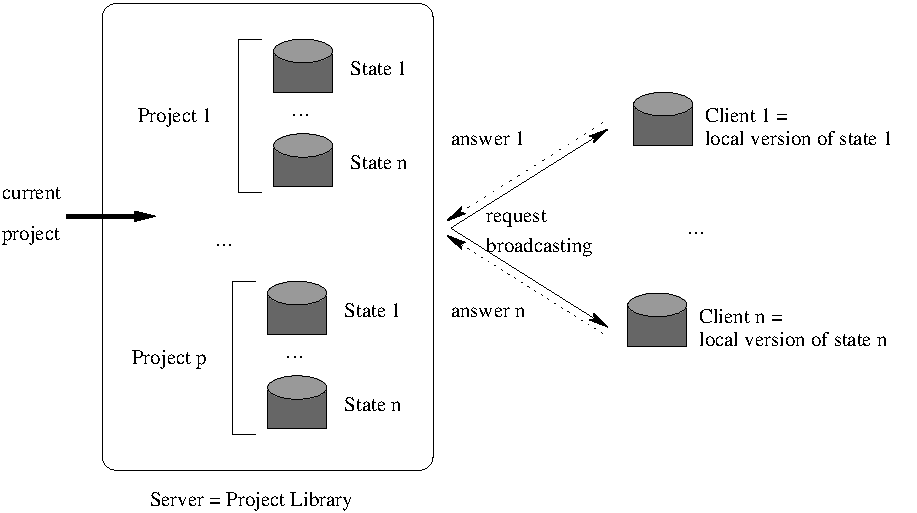
\includegraphics[scale=0.68]{mecanisme.pdf}

  \begin{itemize}
  \item delayed synchronization between client $i$ and server' state $i$
    of the current project    
  \end{itemize}
\end{frame}

%%%%%%%%%%%%%%%%%%%%%%%%%%%%%%%%%%%%%%%%%%%%%%%%%%%%%%%%%%%%%%%%%%%%%%%%%%%%%%%

\subsection{State}

\begin{frame}{State}
  \framesubtitle{Overview}

\begin{itemize}
\item each time you create a global data, ask yourself: "is this data part of a
  project or common to all projects?"
\item most often, it is really part of a project
\item in such cases, you have to create a \emph{projectified state} (otherwise
  use standard \ocaml datastructures like references or hashtables)
\end{itemize}

\end{frame}

%%%%%%%%%%%%%%%%%%%%%%%%%%%%%%%%%%%%%%%%%%%%%%%%%%%%%%%%%%%%%%%%%%%%%%%%%%%%%%%

\begin{frame}[fragile]{State}
  \framesubtitle{Registration Overview}

\begin{itemize}
\item module \lstinline+State_builder+
\item a state is a module created through functor application
\item low-level functor \lstinline+State_builder.Register+
\item several high-level functors
  \begin{itemize}
  \item \lstinline+State_builder.Ref+
  \item \lstinline+State_builder.Option_ref+
  \item \lstinline+State_builder.Set_ref+
  \item \lstinline+State_builder.Hashtbl+
  \item \lstinline+State_builder.Queue+
  \item \lstinline+State_builder.Counter+
  \item ...
  \end{itemize}
\item much simpler to use them (prefer a reference to a record than a mutable
  record, even if less efficient...)
\end{itemize}

\end{frame}

%%%%%%%%%%%%%%%%%%%%%%%%%%%%%%%%%%%%%%%%%%%%%%%%%%%%%%%%%%%%%%%%%%%%%%%%%%%%%%%

\begin{frame}[fragile]{State}
  \framesubtitle{Registration in Practice}

\begin{ocamlcode}
module My_bool_ref = 
  False_ref(struct
    let name = "My_plugin.My_bool_ref"
    let dependencies = []
    let kind = `Correctness
  end)
\end{ocamlcode}

\end{frame}

%%%%%%%%%%%%%%%%%%%%%%%%%%%%%%%%%%%%%%%%%%%%%%%%%%%%%%%%%%%%%%%%%%%%%%%%%%%%%%%

\begin{frame}[fragile]{State}
  \framesubtitle{Registration in Practice (2)}

\begin{ocamlcode}
type callstack = 
  (Cil_types.stmt * Kernel_function.t) list

module My_callstack =
  State_builder.Ref
    (Datatype.List
      (Cil_datatype.Stmt)(Kernel_function))
    (struct 
      let name = "My_plugin.My_callstack"
      let dependencies = 
        [ Ast.self; Kernel_function.self ]
      let kind = `Correctness
      let default () = []
     end)
\end{ocamlcode}

\end{frame}

%%%%%%%%%%%%%%%%%%%%%%%%%%%%%%%%%%%%%%%%%%%%%%%%%%%%%%%%%%%%%%%%%%%%%%%%%%%%%%%

\begin{frame}[fragile]{State}
  \framesubtitle{Registration in Practice (3)}

\begin{ocamlcode}
module My_hashtbl =
  State_builder.Hashtbl
    (Cil_datatype.Stmt.Hashtbl)
    (Datatype.String)
    (struct 
      let name = "My_plugin.My_hashtbl"
      let dependencies = [ Ast.self ]
      let kind = `Correctness
      let size = 17
     end)
\end{ocamlcode}

\end{frame}

%%%%%%%%%%%%%%%%%%%%%%%%%%%%%%%%%%%%%%%%%%%%%%%%%%%%%%%%%%%%%%%%%%%%%%%%%%%%%%%

\begin{frame}[fragile]{State}
  \framesubtitle{Use}

\begin{ocamlcode}
open Cil_types
let _ = object (self)
  inherit Visitor.frama_c_inplace
  method vinst = function
    | Call(_ret_lval, 
           { enode = Lval(Var v, NoOffset) }, 
           _args, 
           _loc) ->
      My_callstack.set
        ((Option.get self#current_stmt,
          Globals.Functions.get v)
        :: (My_callstack.get ()));
      Cil.SkipChildren
    | _ -> Cil.SkipChildren	
end
\end{ocamlcode}

\end{frame}

%%%%%%%%%%%%%%%%%%%%%%%%%%%%%%%%%%%%%%%%%%%%%%%%%%%%%%%%%%%%%%%%%%%%%%%%%%%%%%%

\subsection{Project Operations}

\begin{frame}[fragile]{Project Operations}

  \begin{itemize}
  \item \lstinline+Project.current+
  \item \lstinline+Project.create+, \lstinline+Project.remove+
  \item \lstinline+Project.copy+
  \item \lstinline+Project.save+, \lstinline+Project.load+
  \item  \lstinline+Project.set_current+, \lstinline+Project.on+
\begin{ocamlcode}
let main () =
  let p =
    Sparecode.Register.get
      ~select_annot:false
      ~select_slice_pragma:false
   in
   Project.on p Eva.Analysis.compute ()
\end{ocamlcode}
  \end{itemize}

\end{frame}

%%%%%%%%%%%%%%%%%%%%%%%%%%%%%%%%%%%%%%%%%%%%%%%%%%%%%%%%%%%%%%%%%%%%%%%%%%%%%%%

\subsection{State Selection}

\begin{frame}{State Selection}
  \framesubtitle{Overview}
  \begin{itemize}
  \item project operations may be applied only on some states
  \item such a set of states is called a \emph{state selection}
  \item a way to improve efficiency
  \item a way to easily implement some operations over states (like clearing)
  \item must preserve \framac's global consistency
  \item that is the \emph{raison d'\^etre} of \emph{state dependencies} which
    allows to easily specify consistent selections
  \end{itemize}
\end{frame}

%%%%%%%%%%%%%%%%%%%%%%%%%%%%%%%%%%%%%%%%%%%%%%%%%%%%%%%%%%%%%%%%%%%%%%%%%%%%%%%

\begin{frame}[fragile]{State Selection}
  \framesubtitle{Example}
  
  \begin{ocamlcode}
(* clear value analysis' results
   and all its depending state
   in the current project *)
let selection =
  State_selection.Dynamic.with_dependencies 
    !Db.Value.self
in
Project.clear ~selection ()
  \end{ocamlcode}

\end{frame}

%%%%%%%%%%%%%%%%%%%%%%%%%%%%%%%%%%%%%%%%%%%%%%%%%%%%%%%%%%%%%%%%%%%%%%%%%%%%%%%

\subsection{Marshaling}

\begin{frame}{Marshaling}
\end{frame}


%%%%%%%%%%%%%%%%%%%%%%%%%%%%%%%%%%%%%%%%%%%%%%%%%%%%%%%%%%%%%%%%%%%%%%%%%%%%%%%
%%%%%%%%%%%%%%%%%%%%%%%%%%%%%%%%%%%%%%%%%%%%%%%%%%%%%%%%%%%%%%%%%%%%%%%%%%%%%%%

\part{Writing analyses}

\section{Syntactic analysis}
%VP:1h
\section{Semantic analysis}
%VP:45mn
\section{Manipulating annotations}
%JS:30mn
\begin{frame}[fragile]{Accessing Annotations}

\begin{itemize}
\item do not read annotations directly stored in the AST
\item global annotations: \lstinline+Globals.Annotations+
\item function contracts: \lstinline+Kernel_function.get_spec+
\item code annotations: \lstinline+Annotations+
\item visitor
\end{itemize}

\end{frame}

%%%%%%%%%%%%%%%%%%%%%%%%%%%%%%%%%%%%%%%%%%%%%%%%%%%%%%%%%%%%%%%%%%%%%%%%%%%%%%%

\begin{frame}[fragile]{Generating Annotations}

\begin{itemize}
\item do not modify AST nodes in place
\item copy visitor
\item global annotation: \lstinline+Globals.Annotations.add_generated+
\item function contract: \lstinline+Kernel_function.set_spec+
\item code annotation: \lstinline+Annotations.add+, 
\lstinline+Annotations.add_assert+
\begin{itemize}
\item require a list of states in argument
\item they are the states which the generation of the annotation depends on
\end{itemize}
\begin{ocamlcode}
let value_alarm = ... in
Annotations.add_assert 
  kf stmt [ !Db.Value.self ] value_alarm
\end{ocamlcode}
\end{itemize}

\end{frame}

%%%%%%%%%%%%%%%%%%%%%%%%%%%%%%%%%%%%%%%%%%%%%%%%%%%%%%%%%%%%%%%%%%%%%%%%%%%%%%%

\begin{frame}{Upcoming Annotations}

\begin{itemize}
\item \framac Oxygen provides a fully new API for annotations
\item global annotations, function contracts and code annotations in a single
  module \lstinline+Annotations+
\item new consistent and uniform interface
\item no more states in argument for code annotations
\item but a so-called \emph{emitter} for any new annotation
\end{itemize}

\end{frame}

%%%%%%%%%%%%%%%%%%%%%%%%%%%%%%%%%%%%%%%%%%%%%%%%%%%%%%%%%%%%%%%%%%%%%%%%%%%%%%%

\begin{frame}{Property Statuses}
\framesubtitle{Overview}

\begin{itemize}
\item each plug-in may emit a (local) status for a property $p$, that is
  whether $p$ is valid or invalid
  \begin{itemize}
  \item ``valid'' means: for each execution trace from the beginning on the
    application to $p$, $p$ is  logically valid
  \item ``invalid'' is the opposite of ``valid''
  \item plug-ins must be correct: it cannot says that $p$ is valid
    if it is not (and conversely).
  \end{itemize}
\item the kernel automatically consolidates the result for each property
  according to all emitted statuses
\end{itemize}

\end{frame}

%%%%%%%%%%%%%%%%%%%%%%%%%%%%%%%%%%%%%%%%%%%%%%%%%%%%%%%%%%%%%%%%%%%%%%%%%%%%%%%

\begin{frame}{From Annotations to Properties}
  \framesubtitle{Overview}

\begin{itemize}
\item ACSL annotations may contain several properties (for instance, behaviors)
\item module \lstinline+Property+ defines properties as a single datatype
\item it also provides operations to convert an annotation to a propertie or a
  set of properties
\end{itemize}

\end{frame}

%%%%%%%%%%%%%%%%%%%%%%%%%%%%%%%%%%%%%%%%%%%%%%%%%%%%%%%%%%%%%%%%%%%%%%%%%%%%%%%

\begin{frame}[fragile]{From Annotations to Properties}
  \framesubtitle{Example}

\begin{ocamlcode}
let _ = object
  inherit Visitor.frama_c_inplace as self
  method vcode_annot =
    let ppts = 
      Property.ip_of_code_annot 
        (Option.get self#current_kf)
        (Option.get self#current_stmt)
    in
    Pretty_utils.pp_list "%a" 
      Property.pretty ppts;    
    Cil.SkipChildren	
end
\end{ocamlcode}

\end{frame}

%%%%%%%%%%%%%%%%%%%%%%%%%%%%%%%%%%%%%%%%%%%%%%%%%%%%%%%%%%%%%%%%%%%%%%%%%%%%%%%

\begin{frame}[fragile]{Emitters}

\begin{itemize}
\item emitters emit property statuses according to parameters
\item if a correctness parameter changes, then valid statuses may become invalid
  (or conversely)
\item if a tuning parameter changes, then only unknown statuses may be refined
  into valid or invalid.
\end{itemize}

\begin{ocamlcode}
let emitter = 
  Emitter.create
    "my_emitter"
    ~correctness:[ Kernel.LibEntry.parameter ]
    ~tuning:[ My_tuning_option.paremeter ]
\end{ocamlcode}

\end{frame}

%%%%%%%%%%%%%%%%%%%%%%%%%%%%%%%%%%%%%%%%%%%%%%%%%%%%%%%%%%%%%%%%%%%%%%%%%%%%%%%

\begin{frame}[fragile]{Emitting Statuses}

\begin{ocamlcode}
let () =
  Property_status.emit
    emitter
    ~hyps:[]
    property
    Property.Dont_know
\end{ocamlcode}

\end{frame}

%%%%%%%%%%%%%%%%%%%%%%%%%%%%%%%%%%%%%%%%%%%%%%%%%%%%%%%%%%%%%%%%%%%%%%%%%%%%%%%

\begin{frame}[fragile]{Emitting Statuses}
\framesubtitle{Dependencies}

\begin{itemize}
\item the local status \lstinline+True+ may depend on a set of hypotheses, that
  is other annotations which must be valid to ensure validity
\end{itemize}

\begin{ocamlcode}
let () =
  Property_status.emit
    emitter
    ~hyps:[ Property.ip_lemma "fermat_theorem"]
    property
    Property.True
\end{ocamlcode}

\end{frame}

%%%%%%%%%%%%%%%%%%%%%%%%%%%%%%%%%%%%%%%%%%%%%%%%%%%%%%%%%%%%%%%%%%%%%%%%%%%%%%%

\begin{frame}{Property Statuses}
\framesubtitle{Reachability}

\begin{itemize}
\item ``$p$ is invalid'' means: it exists an execution trace from the beginning
  on the application to $p$ such that $p$ is logically invalid.
\item require a proof of reachability and a proof of invalidity
\item may be difficult
\item 2 different local statuses: 
  \begin{itemize}
  \item \lstinline+False_and_reachable+
  \item \lstinline+False_if_reachable+ which automatically adds an hypothesis
    about reachability of $p$.
  \end{itemize}
\end{itemize}

\end{frame}


\section{Real-world examples}
%VP:45mn

\section{Bibliography}
% reference manuals and articles
\begin{frame}{Bibliography}
  \framesubtitle{Reference Manuals}
  \begin{itemize}
  \item L. Correnson, P. Cuoq, F. Kirchner, V. Prevosto, A. Puccetti,
    J. Signoles and B. Yakobowski. \emph{Frama-C User Manual}. 2011.
  \item P. Baudin, P. Cuoq, J.-C. Filli\^atre, C. March\'e, B. Monate, Y. Moy
    and V. Prevosto. \emph{ACSL: ANSI/ISO C Specification Language}. Version
    1.5. 2011.
  \item J. Signoles, L. Correnson and V. Prevosto. \emph{Frama-C Plug-in
    Development Guide}. 2011.
  \end{itemize}
\end{frame}

\begin{frame}{Bibliography}
  \framesubtitle{Articles}
  \begin{itemize}
  \item P. Cuoq and J. Signoles. \emph{Experience Report: OCaml for an
    Industrial-Strength Static Analysis Framework.} In ICFP 2009.
  \item J. Signoles. \emph{Foncteurs imp\'eratifs et compos\'es: la notion de
    projets dans Frama-C}. In Studia Informatica Universalis. 2009.
  \item J. Signoles. \emph{Une biblioth\`eque de typage dynamique en OCaml.} In
    Studia Informatica Universalis. 2011.
  \item P. Cuoq, D. Doligez and J. Signoles. \emph{Lightweight Typed
    Customizable Unmarshaling}. ML workshop 2011.
  \item L. Correnson and J. Signoles. \emph{Combining Analyses for C Program
    Verification}. To appear in FMICS'12.
  \end{itemize}
\end{frame}


\end{document}

Local Variables:
ispell-local-dictionary: "english"
End:
